\begin{frame}{Content}
    \begin{enumerate}%
      \setlength\itemsep{1em}%
      \item {\color{lightgray} \ti{}} \tei{}
      \item {\color{lightgray} \tii{}} \teii{}
      \item {\color{lightgray} \tiii{}} \teiii{}
      \item {\color{lightgray} \tiv{}} \teiv{}
      \item {\color{lightgray} \tv{}} \tev{}
      \item {\color{lightgray} \tcvi{}} \tevi{}
    \end{enumerate}
  \end{frame}

% \begin{frame}{\tcvi{} Future work}
%     \onslide<2->{
%     \begin{block}{LUCI ES}
%         \begin{itemize}
%             \item Explore ($\mu , \lambda$) ES
%             \item Ranking in Bandit problems
%             \item Heritage (Importance Mixing, elitism)
%             \item Scalability
%         \end{itemize}
%     \end{block}
%     }
%     \onslide<3->{
%     \begin{block}{ES for Policy Search}
%         \begin{itemize}
%             \item Neuroevolution constraints and theory
%             % \item Theory of ES for policy search
%             \item Ablation study of existing methods
%         \end{itemize}
%     \end{block}
%     }
%     \onslide<4->{
%     \begin{block}{Evolving Evolution Strategies}
%         \begin{itemize}
%             \item Make ES methods emerge from scratch
%             % \item Improve current methods by bootstrapping from them
%             \item Neuromodulation: adapting ES during the evolution
%         \end{itemize}
%     \end{block}
%     }
    
% \end{frame}


\begin{frame}{\tcvi{} Future work}%
    \only<1>{
    \begin{block}{LUCI ES}
        \begin{itemize}
            \item Explore ($\mu , \lambda$) ES
            \item Ranking in Bandit problems
            \item Heritage (Importance Mixing, elitism)
            \item Scalability
        \end{itemize}
    \end{block}
    }
    \only<2>{
    \begin{block}{Evolving Evolution Strategies}
        \begin{itemize}
            \item Make ES methods emerge from scratch
            % \item Improve current methods by bootstrapping from them
            \item Neuromodulation: adapting ES during the evolution
        \end{itemize}
    \end{block}
    }
    \only<3>{
    \begin{block}{ES for Policy Search}
        \begin{itemize}
            \item Neuroevolution constraints and theory
            % \item Theory of ES for policy search
            \item Ablation study of existing methods
        \end{itemize}
    \end{block}
    }
    \only<4>{
    }
    \begin{figure}
        \tikzset{every picture/.style={line width=0.75pt}} %set default line width to 0.75pt        

        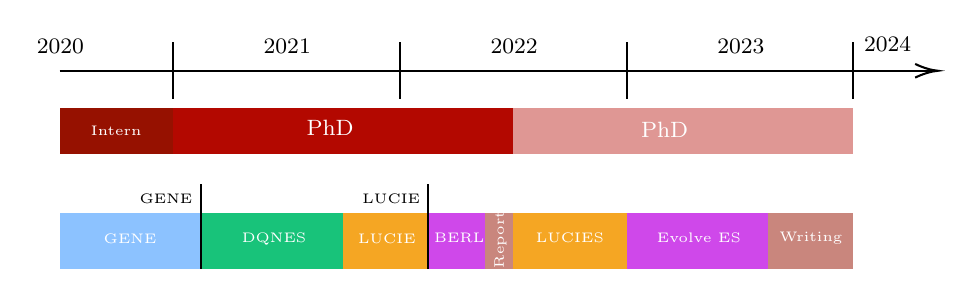
\begin{tikzpicture}[x=0.75pt,y=0.75pt,yscale=-1,xscale=1]
        %uncomment if require: \path (0,300); %set diagram left start at 0, and has height of 300
        
        
        %Straight Lines [id:da263455807473124] 
        \draw    (145.56,104.38) -- (566.71,104.38) ;
        \draw [shift={(568.71,104.38)}, rotate = 180] [color={rgb, 255:red, 0; green, 0; blue, 0 }  ][line width=0.75]    (10.93,-3.29) .. controls (6.95,-1.4) and (3.31,-0.3) .. (0,0) .. controls (3.31,0.3) and (6.95,1.4) .. (10.93,3.29)   ;
        %Straight Lines [id:da06908695747928117] 
        \draw    (200.2,90.72) -- (200.2,118.04) ;
        %Straight Lines [id:da3172970011493099] 
        \draw    (309.48,90.72) -- (309.48,118.04) ;
        %Straight Lines [id:da7182015191619326] 
        \draw    (418.76,90.72) -- (418.76,118.04) ;
        %Straight Lines [id:da5499230746738971] 
        \draw    (528.04,90.72) -- (528.04,118.04) ;
        %Shape: Rectangle [id:dp3072423219363737] 
        \draw  [draw opacity=0][fill={rgb, 255:red, 179; green, 8; blue, 0 }  ,fill opacity=1 ] (200.2,122.14) -- (364.12,122.14) -- (364.12,144.69) -- (200.2,144.69) -- cycle ;
        %Shape: Rectangle [id:dp48101964277359865] 
        \draw  [draw opacity=0][fill={rgb, 255:red, 179; green, 8; blue, 0 }  ,fill opacity=0.42 ] (364.12,122.14) -- (528.04,122.14) -- (528.04,144.69) -- (364.12,144.69) -- cycle ;
        %Shape: Rectangle [id:dp8094283759581382] 
        \draw  [draw opacity=0][fill={rgb, 255:red, 150; green, 17; blue, 0 }  ,fill opacity=1 ] (145.56,122.14) -- (200.2,122.14) -- (200.2,144.69) -- (145.56,144.69) -- cycle ;
        %Shape: Rectangle [id:dp25218225952021045] 
        \draw  [draw opacity=0][fill={rgb, 255:red, 140; green, 194; blue, 255 }  ,fill opacity=1 ] (145.56,172.68) -- (213.86,172.68) -- (213.86,200) -- (145.56,200) -- cycle ;
        %Shape: Rectangle [id:dp439106993654921] 
        \draw  [draw opacity=0][fill={rgb, 255:red, 24; green, 195; blue, 122 }  ,fill opacity=1 ] (213.86,172.68) -- (282.16,172.68) -- (282.16,200) -- (213.86,200) -- cycle ;
        %Shape: Rectangle [id:dp07333800236304988] 
        \draw  [draw opacity=0][fill={rgb, 255:red, 245; green, 166; blue, 35 }  ,fill opacity=1 ] (282.16,172.68) -- (323.14,172.68) -- (323.14,200) -- (282.16,200) -- cycle ;
        %Shape: Rectangle [id:dp055858616927162985] 
        \draw  [draw opacity=0][fill={rgb, 255:red, 150; green, 17; blue, 0 }  ,fill opacity=0.51 ] (350.46,172.68) -- (364.12,172.68) -- (364.12,200) -- (350.46,200) -- cycle ;
        %Shape: Rectangle [id:dp7612465684991917] 
        \draw  [draw opacity=0][fill={rgb, 255:red, 245; green, 166; blue, 35 }  ,fill opacity=1 ] (364.12,172.68) -- (418.76,172.68) -- (418.76,200) -- (364.12,200) -- cycle ;
        %Shape: Rectangle [id:dp6656802192707113] 
        \draw  [draw opacity=0][fill={rgb, 255:red, 207; green, 72; blue, 234 }  ,fill opacity=1 ] (323.14,172.68) -- (350.46,172.68) -- (350.46,200) -- (323.14,200) -- cycle ;
        %Shape: Rectangle [id:dp8472926104883064] 
        \draw  [draw opacity=0][fill={rgb, 255:red, 150; green, 17; blue, 0 }  ,fill opacity=0.51 ] (487.06,172.68) -- (528.04,172.68) -- (528.04,200) -- (487.06,200) -- cycle ;
        %Shape: Rectangle [id:dp6374386242575871] 
        \draw  [draw opacity=0][fill={rgb, 255:red, 207; green, 72; blue, 234 }  ,fill opacity=1 ] (418.76,172.68) -- (487.06,172.68) -- (487.06,200) -- (418.76,200) -- cycle ;
        %Straight Lines [id:da43034538559618607] 
        \draw    (213.86,159.02) -- (213.86,200) ;
        %Straight Lines [id:da5380962385035739] 
        \draw    (323.14,159.02) -- (323.14,200) ;
        %Straight Lines [id:da3604388553748691] 
        % \draw    (418.76,159.02) -- (418.76,200) ;
        
        % Text Node
        \draw (364.53,92.77) node  [font=\footnotesize] [align=left] {2022};
        % Text Node
        \draw (255.25,92.77) node  [font=\footnotesize] [align=left] {2021};
        % Text Node
        \draw (145.97,92.77) node  [font=\footnotesize] [align=left] {2020};
        % Text Node
        \draw (473.81,92.77) node  [font=\footnotesize] [align=left] {2023};
        % Text Node
        \draw (544.5,91.5) node  [font=\footnotesize] [align=left] {2024};
        % Text Node
        \draw (179.54,185.45) node  [font=\tiny,color={rgb, 255:red, 255; green, 255; blue, 255 }  ,opacity=1 ] [align=left] {GENE};
        % Text Node
        \draw (248.92,185.45) node  [font=\tiny,color={rgb, 255:red, 255; green, 255; blue, 255 }  ,opacity=1 ] [align=left] {DQNES};
        % Text Node
        \draw (303.28,185.45) node  [font=\tiny,color={rgb, 255:red, 255; green, 255; blue, 255 }  ,opacity=1 ] [align=left] {LUCIE};
        % Text Node
        \draw (357.97,185.66) node  [font=\fontsize{0.33em}{0.4em}\selectfont,color={rgb, 255:red, 255; green, 255; blue, 255 }  ,opacity=1 ,rotate=-270] [align=left] {Report};
        % Text Node
        \draw (391.44,184.97) node  [font=\tiny,color={rgb, 255:red, 255; green, 255; blue, 255 }  ,opacity=1 ] [align=left] {LUCIES};
        % Text Node
        \draw (338.17,184.97) node  [font=\tiny,color={rgb, 255:red, 255; green, 255; blue, 255 }  ,opacity=1 ] [align=left] {BERL};
        % Text Node
        \draw (507.55,184.97) node  [font=\tiny,color={rgb, 255:red, 255; green, 255; blue, 255 }  ,opacity=1 ] [align=left] {Writing};
        % Text Node
        \draw (453.59,184.97) node  [font=\tiny,color={rgb, 255:red, 255; green, 255; blue, 255 }  ,opacity=1 ] [align=left] {Evolve ES};
        % Text Node
        \draw (196.79,165.85) node  [font=\tiny] [align=left] {GENE};
        % Text Node
        \draw (305.38,165.85) node  [font=\tiny] [align=left] {LUCIE};
        % Text Node
        % \draw (397.59,165.85) node  [font=\tiny] [align=left] {LUCIES};
        % Text Node
        \draw (279.43,131.81) node  [font=\footnotesize,color={rgb, 255:red, 255; green, 255; blue, 255 }  ,opacity=1 ] [align=left] {\begin{minipage}[lt]{22.29pt}\setlength\topsep{0pt}
        PhD
        \end{minipage}};
        % Text Node
        \draw (440.62,132.81) node  [font=\footnotesize,color={rgb, 255:red, 255; green, 255; blue, 255 }  ,opacity=1 ] [align=left] {\begin{minipage}[lt]{22.29pt}\setlength\topsep{0pt}
        PhD
        \end{minipage}};
        % Text Node
        \draw (174.25,133.26) node  [font=\tiny,color={rgb, 255:red, 255; green, 255; blue, 255 }  ,opacity=1 ] [align=left] {\begin{minipage}[lt]{20.36pt}\setlength\topsep{0pt}
        Intern
        \end{minipage}};
        
        \end{tikzpicture}

    \end{figure}
\end{frame}